\documentclass{beamer}
\usepackage[style=authoryear]{biblatex}
\usepackage{mathtools}
\usepackage{tikz,pgfplots}
\addbibresource{references.bib} 
\usetheme{metropolis}
\title{Revenue Maximization for Buyers with Costly Participation}
\date{16.01.2025}
\author{Ayk Borstelmann}
\institute{
    Seminar Algorithmic Game Theory
}

\subtitle{
  \cite{primary}, ACM-SIAM
}

\begin{document}
\maketitle
\section{Introductory Example}
\section{Problem Statement}
\begin{frame}{Problem Statement}
  \onslide<1>{Recall single item auction ...}
  \begin{itemize}
    \item Set $\mathcal{N}$ of $n$ buyers
    \item An item to sell
    \item Each buyer $i \in \mathcal{N}$ has
          \begin{itemize}
            \item private valuation $v_i \in \mathbb{R}_{\geq0}$
            \item<2-> \alert{private participation cost $c_i \in \mathbb{R}$}
          \end{itemize}
    \item Mechanism $\mathcal{M} = (x,p)$
          \begin{itemize}
            \item $x: \mathbb{R} \only<2>{\times \mathbb{R}} \rightarrow [0,1]^n$ Allocation function
            \item $p: \mathbb{R} \only<2>{\times \mathbb{R}} \rightarrow \mathbb{R}^n$ Payment function
          \end{itemize}
    \item Utility
          \begin{align*}
            u_i(v_i\only<2>{, c_i}) = \alt<1>{v_i x_i(v_i) - p_i(v_i)}{\begin{cases}v_i x_i(v_i, c_i) - p_i(v_i, c_i) - \alert{c_i} & \text{i participates} \\ 0 & \text{otherwise}\end{cases}}
          \end{align*}
  \end{itemize}
  \onslide<2>{
    Call $t_i = (v_i, c_i) \sim \bar{F}_i$ the type of a player.
  }
\end{frame}
\section{Single Buyer - Incentive Compatible \& Expected Revenue}

\begin{frame}{Truthful Mechanism - Myerson}
  \begin{lemma}[\cite{myerson}, Single Buyer]
    For single parameter environments, an allocation rule $x$ is implementable if and only if it is monotone.
    If $x$ is monotone, then there exists a unique payment rule $p$, s.t. the mechanism $M=(x,p)$ is truthful
    and $p$ is given by:
    \begin{align*}
      p(v) = v x(v) - \int_0^v x(t) dt + p_0
    \end{align*}
  \end{lemma}
\end{frame}

\begin{frame}{Truthful Mechanism - Private Cost}
  \begin{lemma}[\cite{primary}]
    It is without loss for seller to commit to a truthful single parameter mechanism $\mathcal{M}=(x,p)$ and
    for the buyer to participate and truthfully reveal v if and only if $u^\mathcal{M}(v) = \int_0^v x(z)dz - p_0 \geq c$.
  \end{lemma}
  (Without proof.)
\end{frame}

\begin{frame}{Expected Revenue - Myerson}
  \begin{lemma}[\cite{myerson}, Single Buyer]
    Let $\mathcal{M}=(x,p)$ be a truthful single-parameter mechanism, then the expected revenue equals the expected virtual welfare. That is
    \begin{align*}
      \mathbf{E}_v\left[p(v)\right]
      = \mathbf{E}_v\left[x(v)\varphi(v)\right] + p_0
    \end{align*}

    where $\varphi(t) = t - \frac{1 - F(t)}{f(t)}$
  \end{lemma}
\end{frame}

\begin{frame}{Truthful Mechanism - Private Cost}
  Given any single parameter truthful mechanism $\mathcal{M} = (x,p)$ (without respecting private cost $c$).

  \begin{columns}<2->
    \begin{column}{.5\textwidth}
      \begin{align*}
        v_x(c) & = \inf_{v \in \mathbb{R}_{\geq 0}} \{\underbrace{v x(v) - p(v)}_{u^\mathcal{M}(v)} \geq c\} \\
      \end{align*}
    \end{column}
    \begin{column}{.5\textwidth}
      \begin{tikzpicture}
        \draw (0,0) -- (2.5,0) node[right] {\( c \)};
        \draw (0,0) -- (0,2.5) node[above] {\( v_x(c) \)};

        \draw[thick,domain=0:2] plot (\x,{0.5+\x});
      \end{tikzpicture}
    \end{column}
  \end{columns}

  \begin{columns}<3->
    \begin{column}{.5\textwidth}
      \begin{align*}
        x_c(v) & = \begin{cases}
                     x(v) & v \geq v_x(c) \\
                     0    & v < v_x(c)
                   \end{cases}
      \end{align*}
    \end{column}
    \begin{column}{.5\textwidth}
      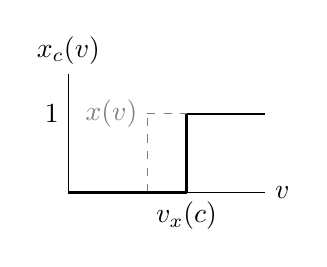
\begin{tikzpicture}
        \draw (0,0) -- (2.5,0) node[right] {$v$};
        \draw (0,0) -- (0,1.5) node[above] {$x_c(v)$};

        \draw[dashed, gray] (0,0) -- (1,0);
        \draw[dashed, gray] (1,1) -- (2.5,1);
        \draw[dashed, gray] (1,0) -- (1,1);

        \draw[thick] (0,0) -- (1.5,0);
        \draw[thick] (1.5,1) -- (2.5,1);
        \draw[thick] (1.5,0) -- (1.5,1);
        \node[below] at (1.5,0) {$v_x(c)$};

        \node[left] at (0,1) {$1$};
        \node[left, gray] at (1,1) {$x(v)$};
      \end{tikzpicture}

    \end{column}
  \end{columns}
\end{frame}

\begin{frame}{Expected Revenue - Private Cost}
  $\bar{F}_c$: conditional \textbf{value} distribution, when participation cost is $c$
  \begin{align*}
    \varphi_c(v) = v - \frac{1- \bar{F}_c(v)}{\hat{f}_c(v)}
  \end{align*}

  \begin{theorem}<2->[\cite{primary}]
    Given any $\bar{F}$ with marginal cost distribution $G$, any mechanism $\mathcal{M}=(x,p)$, then the expected revenue $\mathbf{E}_{t \sim \bar{F}}\left[p_c(v)\right]$ of the seller is

    \begin{align*}
      \mathbf{E}_{c \sim G}\left[\mathbf{E}_{v\sim\bar{F}_c}\left[x_c(v)\varphi_c(v)\right] - (1-\bar{F}_c(v_x(c))) \cdot \max\{-p_0,c\}\right]
    \end{align*}
  \end{theorem}
\end{frame}

\begin{frame}{Expected Revenue - Private Cost - Example}
  \begin{example}
    For $c = 0$, i.e., $G$, s.t. $\mathbf{Pr}_{c \sim G}[c = 0] = 1$ and $p_0 = 0$:
  \end{example}

  Then
  \begin{itemize}
    \item<2-> $\varphi_c(v) = \varphi(v)$
    \item<3-> $\bar{F}_c(v) = \bar{F}(v)$
    \item<4-> $\mathbf{E}_{v \sim F}\left[x_c(v) \varphi_c(v)\right] = \mathbf{E}_{v \sim F}\left[x(v) \varphi(v)\right]$
      (individual rationality if $p_0 = 0$)
  \end{itemize}

  \onslide<5->{
    \begin{align*}
      \Rightarrow & \mathbf{E}_{c \sim G}\left[\mathbf{E}_{v\sim\bar{F}_c}\left[x_c(v)\varphi_c(v)\right] - (1-\bar{F}_c(v_x(c))) \cdot \underbrace{\max\{-p_0,c\}}_{=0}\right] \\
      =           & \mathbf{E}_{v \sim \bar{F}}\left[x(v) \varphi(v)\right]
    \end{align*}
  }
\end{frame}

\begin{frame}{Expected Revenue - Private Cost - Proof}
  \textbf{Proof.}\\

  Let $c$ be fixed arbitrarily.

  Case $c > -p_0$ $\Rightarrow$ $v_x(c) > 0$ \\
  \begin{itemize}
    \item<2-> If player participates [$v \geq v_x(c)$]\\
      $p_c(v) = v x(v) - \int_0^vx(t)dt + p_0 = v x_{\alert{c}}(v) - \int_0^v x_{\alert{c}}(v) \alert{- c}$ \\
    \item<3-> If player opts out [$v < v_x(c)$]\\
      $p_c(v) = 0 = v x_c(v) - \int_0^v x_c(t) dt$
  \end{itemize}

  \onslide<4->{
    \begin{align*}
      \mathbf{E}_{v \sim \bar{F}_c}\left[p_c(v)\right] & = \mathbf{E}_{v \sim \bar{F}_c}\left[v \cdot x_c(v) - \int_0^v x_c(t)dt - c \cdot \mathbf{1}\left[v \geq v_x(c)\right]\right] \\
      \onslide<5->{                                    & = \mathbf{E}_{v \sim \bar{F}_c}\left[x_c(v)\varphi_c(v)\right] - (1 - \bar{F}_c(v_x(c))) \cdot c}
    \end{align*}
  }

\end{frame}
\begin{frame}{Expected Revenue - Private Cost - Proof (Cont.)}

  Case $c \leq -p_0$ $\Rightarrow$ $v_x(c) = 0$ \\
  \begin{itemize}
    \item<2-> Player participates \\
      $p_c(v) = v x(v) - \int_0^vx(t)dt + p_0 = v x_c(v) - \int_0^v x_c(v) + p_0$ \\
  \end{itemize}

  \onslide<3->{
    \begin{align*}
      \mathbf{E}_{v \sim \bar{F}_c}\left[p(v)\right] & = \mathbf{E}_{v \sim \bar{F}_c} \left[v x_c(v) - \int_0^v x_c(v) + p_0 \right]                                               \\
      \onslide<4->{                                  & = \mathbf{E}_{v \sim \bar{F}_c}\left[x_c(v)\varphi_c(v)\right] + p_0                               \\}
      \onslide<5->{                                  & = \mathbf{E}_{v \sim \bar{F}_c}\left[x_c(v)\varphi_c(v)\right] + (1 - \bar{F}_c(v_x(c))) \cdot p_0}
    \end{align*}
  }

\end{frame}
\begin{frame}{Expected Revenue - Private Cost - Proof (Cont.)}

  Case $c > -p_0$ + Case $c \leq -p_0$
  \begin{align*}
    \Rightarrow    & \mathbf{E}\left[p_c(v)\right]                                                                                                           \\
    \onslide<2->{= & \mathbf{E}_{c \sim G}\left[\mathbf{E}_{v \sim \bar{F}_c}\left[x_c(v)\varphi_c(v)\right] + (1-\bar{F}_c(v_x(c))) \max\{c, -p_0\}\right]}
  \end{align*}

  \qed
\end{frame}

\section{Single Buyer - Revenue Maximizing Mechanism}

\begin{frame}{FPTAS Algorithm - Motivation}
  Search for $\operatorname{argmax}_{\mathcal{M}} \mathbf{E}\left[p_c(v)\right]$.

  But: $\mathbf{E}\left[p_c(v)\right]$ is non-convex.

  $\Rightarrow$ Approximate $\operatorname{argmax}_{\mathcal{M}} \mathbf{E}\left[p_c(v)\right]$ using FPTAS.

  \textbf{Idea}:
  \begin{itemize}
    \item Normalize $v$ to $[0,1]$
    \item Discretize value $v$'s and allocation function $x$'s space.
    \item Calculate optimal discretized mechanism $\mathcal{M}'$, i.e., optimal allocation function $x(v)$ for each $v$.
  \end{itemize}

\end{frame}

\begin{frame}{FPTAS Algorithm - Dynamic Programming}
  For $v \in [0,1]$
  \begin{itemize}
    \item<1-> Let $\epsilon \in (0,1)$ (discretization degree).
    \item<2-> Let $\bar{F}'$ be type distribution of $\bar{F}$ with \textbf{value} rounded down to nearest multiple of $\epsilon$.
    \item<3-> Round allocation function down to the nearest multiple of $\epsilon$
  \end{itemize}

  \alt<4>{
    Idea: Partially fix mechanism and optimize rest later $\rightarrow$ Dynamic Programming
    \begin{align*}
      \max_{\mathcal{M}'} \mathbf{E}_{t \sim \bar{F}'}\left[p_c(v)\right] & = \max_{j, k} \max_{\mathcal{M}' : x(i\epsilon) = j\epsilon, u(i\epsilon) = k \epsilon^2}\mathbf{E}_{t \sim \bar{F}'}\left[p_c(v)\right] \\
                                                                          & = \max_{j, k} R(1 / \epsilon, j, k)
    \end{align*}
  }{
    \begin{center}
      \begin{tikzpicture}[>=latex]
        \begin{axis}[
            width=.5\textwidth,
            height=.5\textwidth,
            xlabel={$v$},
            ylabel={$x(v)$},
            grid=major,
            xtick={0,0.4,0.6,0.8,1},
            ytick={0,0.4,0.6,0.8,1},
            extra x ticks={0.2},
            extra x tick labels={$\epsilon$},
            extra y ticks={0.2},
            extra y tick labels={$\epsilon$},
            xmin=0, xmax=1, ymin=0, ymax=1,
            domain=0:1,
          ]
          % Horizontal line at y = 0.2
          \addplot[blue] {x^2};

          \only<2->{
            \addplot[domain=0:1,thick,dotted,samples=1000] {floor(5*x) / 5)^2};
          }

          \only<3->{
            \addplot[domain=0:1,thick,samples=1000] {floor(5*(floor(5*x) / 5)^2)/5};
          }
        \end{axis}
      \end{tikzpicture}
    \end{center}
  }
\end{frame}

\begin{frame}{Dynamic Programming - Recursive Formula}
  Where $R(i,j,k)$ be the optimal revenue from buyers
  \begin{itemize}
    \item with $v \leq i \cdot \epsilon$ with $i \leq \frac{1}{\epsilon}$
    \item where $x(i \cdot \epsilon) = j \cdot \epsilon$ with $j \leq \frac{1}{\epsilon}$
    \item and $u(i \cdot \epsilon) = k \cdot \epsilon^2$ with $k \leq \frac{1}{\epsilon^2}$
  \end{itemize}
  \begin{align*}
    \max_{\mathcal{M}' : x(i\epsilon) = j\epsilon, u(i\epsilon) = k\epsilon^2} \mathbf{Pr}[v \leq i \epsilon] \mathbf{E}[p_c(v) \mid v \leq i \epsilon] = R(i,j,k)
  \end{align*}

  \textbf{Base case:}
  For $i = 1$ we have
  \begin{itemize}
    \item $R(1,j,k) = 0$ for any $k \leq j$
    \item $R(1,j,k) = -\infty$ for $k > j$
  \end{itemize}
\end{frame}

\begin{frame}{Dynamic Programming - Recursive Step}
  \textbf{Recursion Step:}
  Let $i \geq 2$.
  \begin{align*}
     & R(i,j,k)                                                                                                                                     \\
     & = \max_{\mathcal{M}' : x(i\epsilon) = j\epsilon, u(i\epsilon) = k\epsilon^2}
    \mathbf{Pr}[v \leq i \epsilon] \alert<2>{\mathbf{E}\left[p_c(v) \mid v \leq i \epsilon\right]}                                                  \\
    \onslide<3-8>{
     & = \alert<8>{\max_{\mathcal{M}' : x(i\epsilon) = j\epsilon, u(i\epsilon) = k\epsilon^2}}
    \only<-4>{\alert<4>{\mathbf{Pr}[v \leq i \epsilon]}} \big(                                                                                      \\
     & \quad \only<5-6>{\alert{\mathbf{Pr}[v \leq i \epsilon]}} \alert<6,7,8>{\mathbf{Pr}[v \leq (i-1) \epsilon \only<-4>{\mid v \leq i \epsilon}]}
    \alert<8>{\mathbf{E}\left[p_c(v) \mid v \leq (i - 1) \epsilon\right]}                                                                           \\
     & \quad + \only<5-6>{\alert{\mathbf{Pr}[v \leq i \epsilon]}} \alert<6,7>{\mathbf{Pr}[v = i\epsilon \only<-4>{\mid v \leq i \epsilon}]}
    \mathbf{E}\left[p_c(v) \mid v = i\epsilon\right]                                                                                                \\
     & \quad\big)
    }
  \end{align*}
\end{frame}

\begin{frame}<1-9>{Dynamic Programming - Recursive Step - Lower Value}
  \begin{align*}
                  & \max_{\mathcal{M}' : x(i\epsilon) = j\epsilon, u(i\epsilon) = k\epsilon^2} \mathbf{Pr}[v \leq (i-1)\epsilon] \mathbf{E}\left[p_c(v) \mid v \leq (i - 1) \epsilon\right] \\
    \onslide<2->{ & = \max_{\alt<-7>{?}{j' \leq j}} R(i-1, \alt<-7>{\alert<6>{?}}{j'}, \alt<-4>{\alert<3>{?}}{k-j})}
  \end{align*}

  \onslide<4-> {
    \alt<-8>{
      \begin{itemize}
        \item $u((i-1)\epsilon) = \alt<-4>{\alert<4>{?}}{(k-j)\epsilon^2}$
              \only<4>{
                \begin{align*}
                  u(i\epsilon)     & = u((i-1)\epsilon) + \epsilon x(i\epsilon) = u((i-1)\epsilon) + j \epsilon^2 \\
                                   & \Leftrightarrow                                                              \\
                  u((i-1)\epsilon) & = u(i\epsilon) - j \epsilon^2 = k \epsilon2 - j \epsilon^2= (k-j)\epsilon^2
                \end{align*}
              }
        \item<7-> $x((i-1) \epsilon) \leq x(i \epsilon) = j \epsilon$ (x should be monotone)
      \end{itemize}
    }
    {
      \begin{center}
        \begin{tikzpicture}[
            node/.style={circle, draw=black, fill=gray!20, scale=.4},
            axis/.style={->, thick},
            gridline/.style={gray, dashed}
          ]

          \draw[axis] (0, 0) -- (3.5, 0) node[right] {$i$};
          \draw[axis] (0, 0) -- (0, 3.5) node[above] {$j$};

          \foreach \x in {1, 2, 3} {
              \draw[gridline] (\x, 0) -- (\x, 3.5);
              \draw[gridline] (0, \x) -- (3.5, \x);
            }

          \foreach \i in {1, 2, 3} {
              \foreach \j in {1, 2, 3} {
                  \ifthenelse{\i=3\and\j=2}
                  {
                    \node[node, fill=green!20] at (\i, \j) {$R(\i,\j,k)$};
                  }
                  {
                    \ifthenelse{\i=2\and\j<3}
                    {
                      \node[node, fill=blue!20] at (\i, \j) {$R(\i,\j,k)$};
                    }
                    {
                      \node[node] at (\i, \j) {$R(\i,\j,k)$};
                    }
                  }
                }
            }

          \node at (0, 0) [below left] {0};
          \foreach \x in {1, 2, 3, 3} {
              \node at (0, \x) [left] {\x};
              \node at (\x, 0) [below] {\x};
            }
        \end{tikzpicture}
      \end{center}
    }
  }
\end{frame}

\begin{frame}<-3>{Dynamic Programming - Recursive Step}
  \textbf{Recursion Step:}
  Let $i \geq 2$.
  \begin{align*}
     & R(i,j,k)                                                                                                                                               \\
    \alt<1>{
     & = \max_{\mathcal{M}' : x(i\epsilon) = j\epsilon, u(i\epsilon) = k\epsilon^2} \big(                                                                     \\
     & \quad \mathbf{Pr}[v \leq (i-1) \epsilon] \mathbf{E}\left[p_c(v) \mid v \leq (i - 1) \epsilon\right]                                                    \\
    }{
     & = \max_{j' \leq j} R(i-1, j', k-j)                                                                                                                     \\
    }
     & \quad + \alert<3>{\mathbf{Pr}[v = i\epsilon] \mathbf{E}\left[p_c(v) \mid v = i\epsilon\right]_{x(i\epsilon) = j\epsilon, u(i\epsilon) = k \epsilon^2}} \\
    \only<1>{
     & \quad\big)
    }
  \end{align*}
\end{frame}

\begin{frame}{Dynamic Programming - Recursive Step - Exact value}
  Occurrence Probability
  \begin{align*}
    \mathbf{Pr}[v = i\epsilon] \eqcolon q_i
  \end{align*}

  \onslide<2-> {
    Expected Revenue given that $v = i \epsilon$, $x(i\epsilon) = j\epsilon$ and $u(i\epsilon)=k\epsilon^2$
    \begin{align*}
       & \mathbf{E}\left[p_c(v) \mid v = i\epsilon\right]_{x(i\epsilon) = j\epsilon, u(i\epsilon) = k \epsilon^2}                                                          \\
      \onslide<3->{
       & = \mathbf{Pr}[c \leq u(i \epsilon)] \cdot \mathbf{E}\left[p_c(i\epsilon) \mid c \leq u(i\epsilon) \right]_{x(i\epsilon) = j\epsilon, u(i\epsilon) = k \epsilon^2} \\
      }
      \onslide<4->{
       & = \bar{F}'_i(k \epsilon^2) \cdot \mathbf{E}\left[p(i \epsilon)\right]_{x(i\epsilon) = j\epsilon, u(i\epsilon) = k \epsilon^2}
      }
    \end{align*}
  }
  \onslide<5->{
    Payment When Participating
    \begin{align*}
      p(v) = u(v) - v x(v) \onslide<6->{= k\epsilon^2 - i \cdot \epsilon \cdot j \cdot \epsilon = (i \cdot j - k) \epsilon^2}
    \end{align*}
  }
\end{frame}

\begin{frame}{Dynamic Programming - Recursive Step}
  \textbf{Recursion Step:}
  Let $i \geq 2$.
  \begin{align*}
     & R(i,j,k)
    \only<-1>{
    \\
     &
    }
    = \max_{j' \leq j} R(i-1, j', k-j)
    \alt<-1>{
    \\
     & \quad + \alert<3>{\mathbf{Pr}[v = i\epsilon] \mathbf{E}\left[p_c(v) \mid v = i\epsilon\right]_{x(i\epsilon) = j\epsilon, u(i\epsilon) = k \epsilon^2}} \\
    }{
    + q_i \cdot \bar{F_i}'(k \cdot \epsilon^2) \cdot (i\cdot j - k) \epsilon^2                                                                                \\
    }
  \end{align*}
\end{frame}

\begin{frame}{Dynamic Programming - Recursive Formula}
  \begin{columns}
    \begin{column}{.6\textwidth}
      $R(i,j,k)$ : optimal revenue from buyers
      \begin{itemize}
        \item with $v \leq i \cdot \epsilon$ with $i \leq \frac{1}{\epsilon}$
        \item where $x(i \cdot \epsilon) = j \cdot \epsilon$ with $j \leq \frac{1}{\epsilon}$
        \item and $u(i \cdot \epsilon) = k \cdot \epsilon^2$ with $k \leq \frac{1}{\epsilon^2}$
      \end{itemize}

      \textbf{Base case:}
      For $i = 1$ we have
      \begin{itemize}
        \item $R(1,j,k) = 0$ for any $k \leq j$
        \item $R(1,j,k) = -\infty$ for $k > j$
      \end{itemize}

      \textbf{Recursion Step:}
      For $i \geq 2$, we have
      \begin{align*}
        R(i,j,k) = & \max_{j' \leq j} R(i-1, j', k-j) \\ &+ q_i \cdot \bar{F_i}'(k \cdot \epsilon^2)\cdot (i \cdot j - k)\epsilon^2
      \end{align*}
    \end{column}
    \begin{column}{.4\textwidth}
      \begin{center}
        \begin{tikzpicture}[
            node/.style={circle, draw=black, fill=gray!20, scale=.4},
            axis/.style={->, thick},
            gridline/.style={gray, dashed}
          ]

          \draw[axis] (0, 0) -- (3.5, 0) node[right] {$i$};
          \draw[axis] (0, 0) -- (0, 3.5) node[above] {$j$};

          \foreach \x in {1, 2, 3} {
              \draw[gridline] (\x, 0) -- (\x, 3.5);
              \draw[gridline] (0, \x) -- (3.5, \x);
            }

          \foreach \i in {1, 2, 3} {
              \foreach \j in {1, 2, 3} {
                  \ifthenelse{\i=3\and\j=2}
                  {
                    \node[node, fill=green!20] at (\i, \j) {$R(\i,\j,k)$};
                  }
                  {
                    \ifthenelse{\i=2\and\j<3}
                    {
                      \node[node, fill=blue!20] at (\i, \j) {$R(\i,\j,k)$};
                    }
                    {
                      \node[node] at (\i, \j) {$R(\i,\j,k)$};
                    }
                  }
                }
            }

          \node at (0, 0) [below left] {0};
          \foreach \x in {1, 2, 3, 3} {
              \node at (0, \x) [left] {\x};
              \node at (\x, 0) [below] {\x};
            }
        \end{tikzpicture}
      \end{center}
    \end{column}
  \end{columns}
\end{frame}

\begin{frame}{FPTAS Algorithm}
  Optimal revenue $\mathcal{M}'$ on discretized value and allocation function space:
  \begin{align*}
    \max_{\mathcal{M}'} \mathbf{E}\left[p_c(v)\right] = \max_{j,k} R(1/\epsilon, j, k)
  \end{align*}

  \begin{theorem}[\citeauthor{primary}]
    For any distribution $\bar{F}$ supported on $[0,1]^2$, for any $\epsilon \in (0,1)$ the algorithm computes a mechanism with revenue of at least $OPT(\bar{F}) - 4\epsilon$ in $O(\frac{1}{\epsilon^5})$ time.
  \end{theorem}
\end{frame}

\begin{frame}{FPTAS Algorithm - Proof}
  \textbf{Proof.}\\
  \begin{align*}
    \mathrm{Rev}(\bar{F}, \mathcal{M}') & \geq \mathrm{Rev}(\bar{F}', \mathcal{M}')
    \onslide<2-> {
    \\ &\geq \mathrm{Rev}(\bar{F}', \widehat{\mathcal{M}}) - \epsilon = \mathrm{OPT}(\bar{F}') - \epsilon
    }
    \onslide<3>{
    \\ &\geq \mathrm{OPT}(\bar{F}) - 4 \epsilon
    }
  \end{align*}
  \onslide<3>{\qed}

  \onslide<2->{
    \alt<2>{
      Where $\widehat{\mathcal{M}}$ is the optimal mechanism on $\bar{F}'$ (allocation rule not necessarily discretized).

      \begin{lemma}[\cite{primary}]
        For any distribution $\bar{F}$ supported on $[0,1]^2$ and for any pair of mechanisms $\mathcal{M}'$ and $\widehat{\mathcal{M}}$
        with allocation rules $x'$ and $\hat{x}$, s.t. $x'(v) \in [\hat{x}(v), \hat{x}(v) + \epsilon]$ for all $\epsilon$, we have $\mathrm{Rev}(\bar{F}, \mathcal{M}') \geq \mathrm{Rev}(\bar{F}, \widehat{\mathcal{M}}) - \epsilon$.
      \end{lemma}
    }{
      \begin{lemma}[\cite{primary}]
        Let $(\Omega, \mathcal{F}, P)$ be any probability measure and let $t_1, t_2: \Omega \rightarrow \mathbb{R}^2$ be two 2-dimensional random variables.
        If $\sup_{\omega \in \Omega} || t_1(\omega) - t_2(\omega) ||_\infty \leq \epsilon$, then $|\mathrm{OPT}(t_1) - \mathrm{OPT}(t_2)| \leq 3\epsilon$.
      \end{lemma}
    }
  }
\end{frame}

\section{Multiple Buyers}

\begin{frame}{Multiple Buyers}
  How can we use the single buyer mechanism for multiple buyers ?
  \textbf{Idea: Ex-Ante Allocation Constraints}
  \begin{itemize}
    \item Restrict each mechanism to only allocate the item to buyer $i$ in expectation with probability $q_i$
    \item Approach each buyer sequentially and execute restricted mechanism (as long as not yet sold)
  \end{itemize}

  $\Rightarrow$ Sequential-opt-out mechanism
\end{frame}

\section{Conclusion}
\begin{frame}{Conclusion}
  \begin{itemize}
    \item Generalize single item auction to use private costs
    \item Characterize truthful mechanism
    \item Derived expected revenue for such a mechanism
    \item Due to non-convexity, FPTAS to optimize revenue
    \item Use generalized FPTAS for sequential-opt-out mechanism in multiple buyers case
  \end{itemize}
\end{frame}

\begin{frame}{References}
  \printbibliography[heading=none]
\end{frame}

\section{Questions}

\end{document}